% This file was created with tikzplotlib v0.10.1.
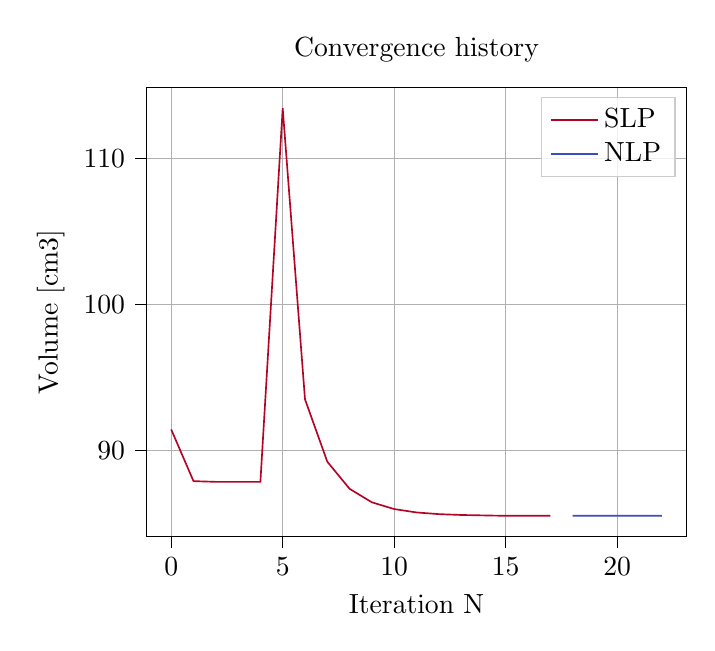
\begin{tikzpicture}

\definecolor{darkgray176}{RGB}{176,176,176}
\definecolor{firebrick180438}{RGB}{180,4,38}
\definecolor{lightgray204}{RGB}{204,204,204}
\definecolor{royalblue5976192}{RGB}{59,76,192}

\begin{axis}[
legend cell align={left},
legend style={fill opacity=0.8, draw opacity=1, text opacity=1, draw=lightgray204},
tick align=outside,
tick pos=left,
title={Convergence history},
x grid style={darkgray176},
xlabel={Iteration N},
xmajorgrids,
xmin=-1.1, xmax=23.1,
xtick style={color=black},
y grid style={darkgray176},
ylabel={Volume [cm3]},
ymajorgrids,
ymin=84.1404966321329, ymax=114.805744147275,
ytick style={color=black}
]
\addplot [semithick, firebrick180438]
table {%
0 91.4425585116738
1 87.9070802673692
2 87.8579447685309
3 87.8579100270034
4 87.8579100269807
5 113.411869260223
6 93.5050018496608
7 89.2353746151231
8 87.3815440623512
9 86.4579648560041
10 85.9961760131869
11 85.765281682217
12 85.6498296002172
13 85.5921081534132
14 85.5632480255216
15 85.5343722417418
16 85.5343878951324
17 85.5343878951312
};
\addlegendentry{SLP}
\addplot [semithick, royalblue5976192]
table {%
18 85.5343878920017
19 85.5343715191848
20 85.5343876965408
21 85.5343879780248
22 85.5343879791021
};
\addlegendentry{NLP}
\end{axis}

\end{tikzpicture}
